\subsection{Ultraschallmodul HC-SR04}
Das Ultraschallmodul HC-SR04 ist ein sehr verbreitetes Modul. Die Popularität
dieses Moduls ist gegeben durch die folgenden Eigenschaften:
\begin{itemize}
	\item unteres Preissegment (<30 CHF)
	\item Mittlerer Messbereich (2 - 400cm)
	\item Digitales Interface (TTL)
	\item Geringer Energiebedarf (75mW)
	\item Einfache Ansteuerung
\end{itemize}

\subsubsection{Prüfeinrichtung}
Für die Prüfung des Ultraschallmoduls ist ein projektnahes Umfeld erstellt 
worden im Elektroniklabor B332b. Hierzu ist ein freistehender Tisch aufgestellt
worden in Richtung des Ultraschallmoduls. Auf diesem ist ein passender Eimer
platziert worden. Dieser hat die folgenden Eckdaten:

\begin{table}[h!]
	\centering
	\begin{tabular}{l l}
		Eigenschaft		& Wert \\
		\hline
		Durchmesser oben	& 38cm \\
		Durchmesser unten	& 33cm \\
		Höhe 			& 48cm \\
		Farbe 			& Schwarz (matt) \\
		Material		& Kunststoff \\
		Hersteller		& Helit \\
		Typ			& 61062
	\end{tabular}
	\caption{Testeimer Eckdaten}
	\label{tab:testeimer}
\end{table}

Um auch eine gewisse Relevanz und statistische Macht zu erreichen, sind 
sämtliche Prüfungen auch statistisch analysiert worden mit mindestens tausend
Einzelmessungen. Hierzu sind die Geräte des Elektroniklabor verwendet worden.
Dabei diente ein Frequenzgenerator als Ansteuerung und ein Digitales 
Speicheroszilloskop als Messmittel, welches auch gleich die statistischen 
Daten berechnete.

\begin{figure}[h!]
	\centering
		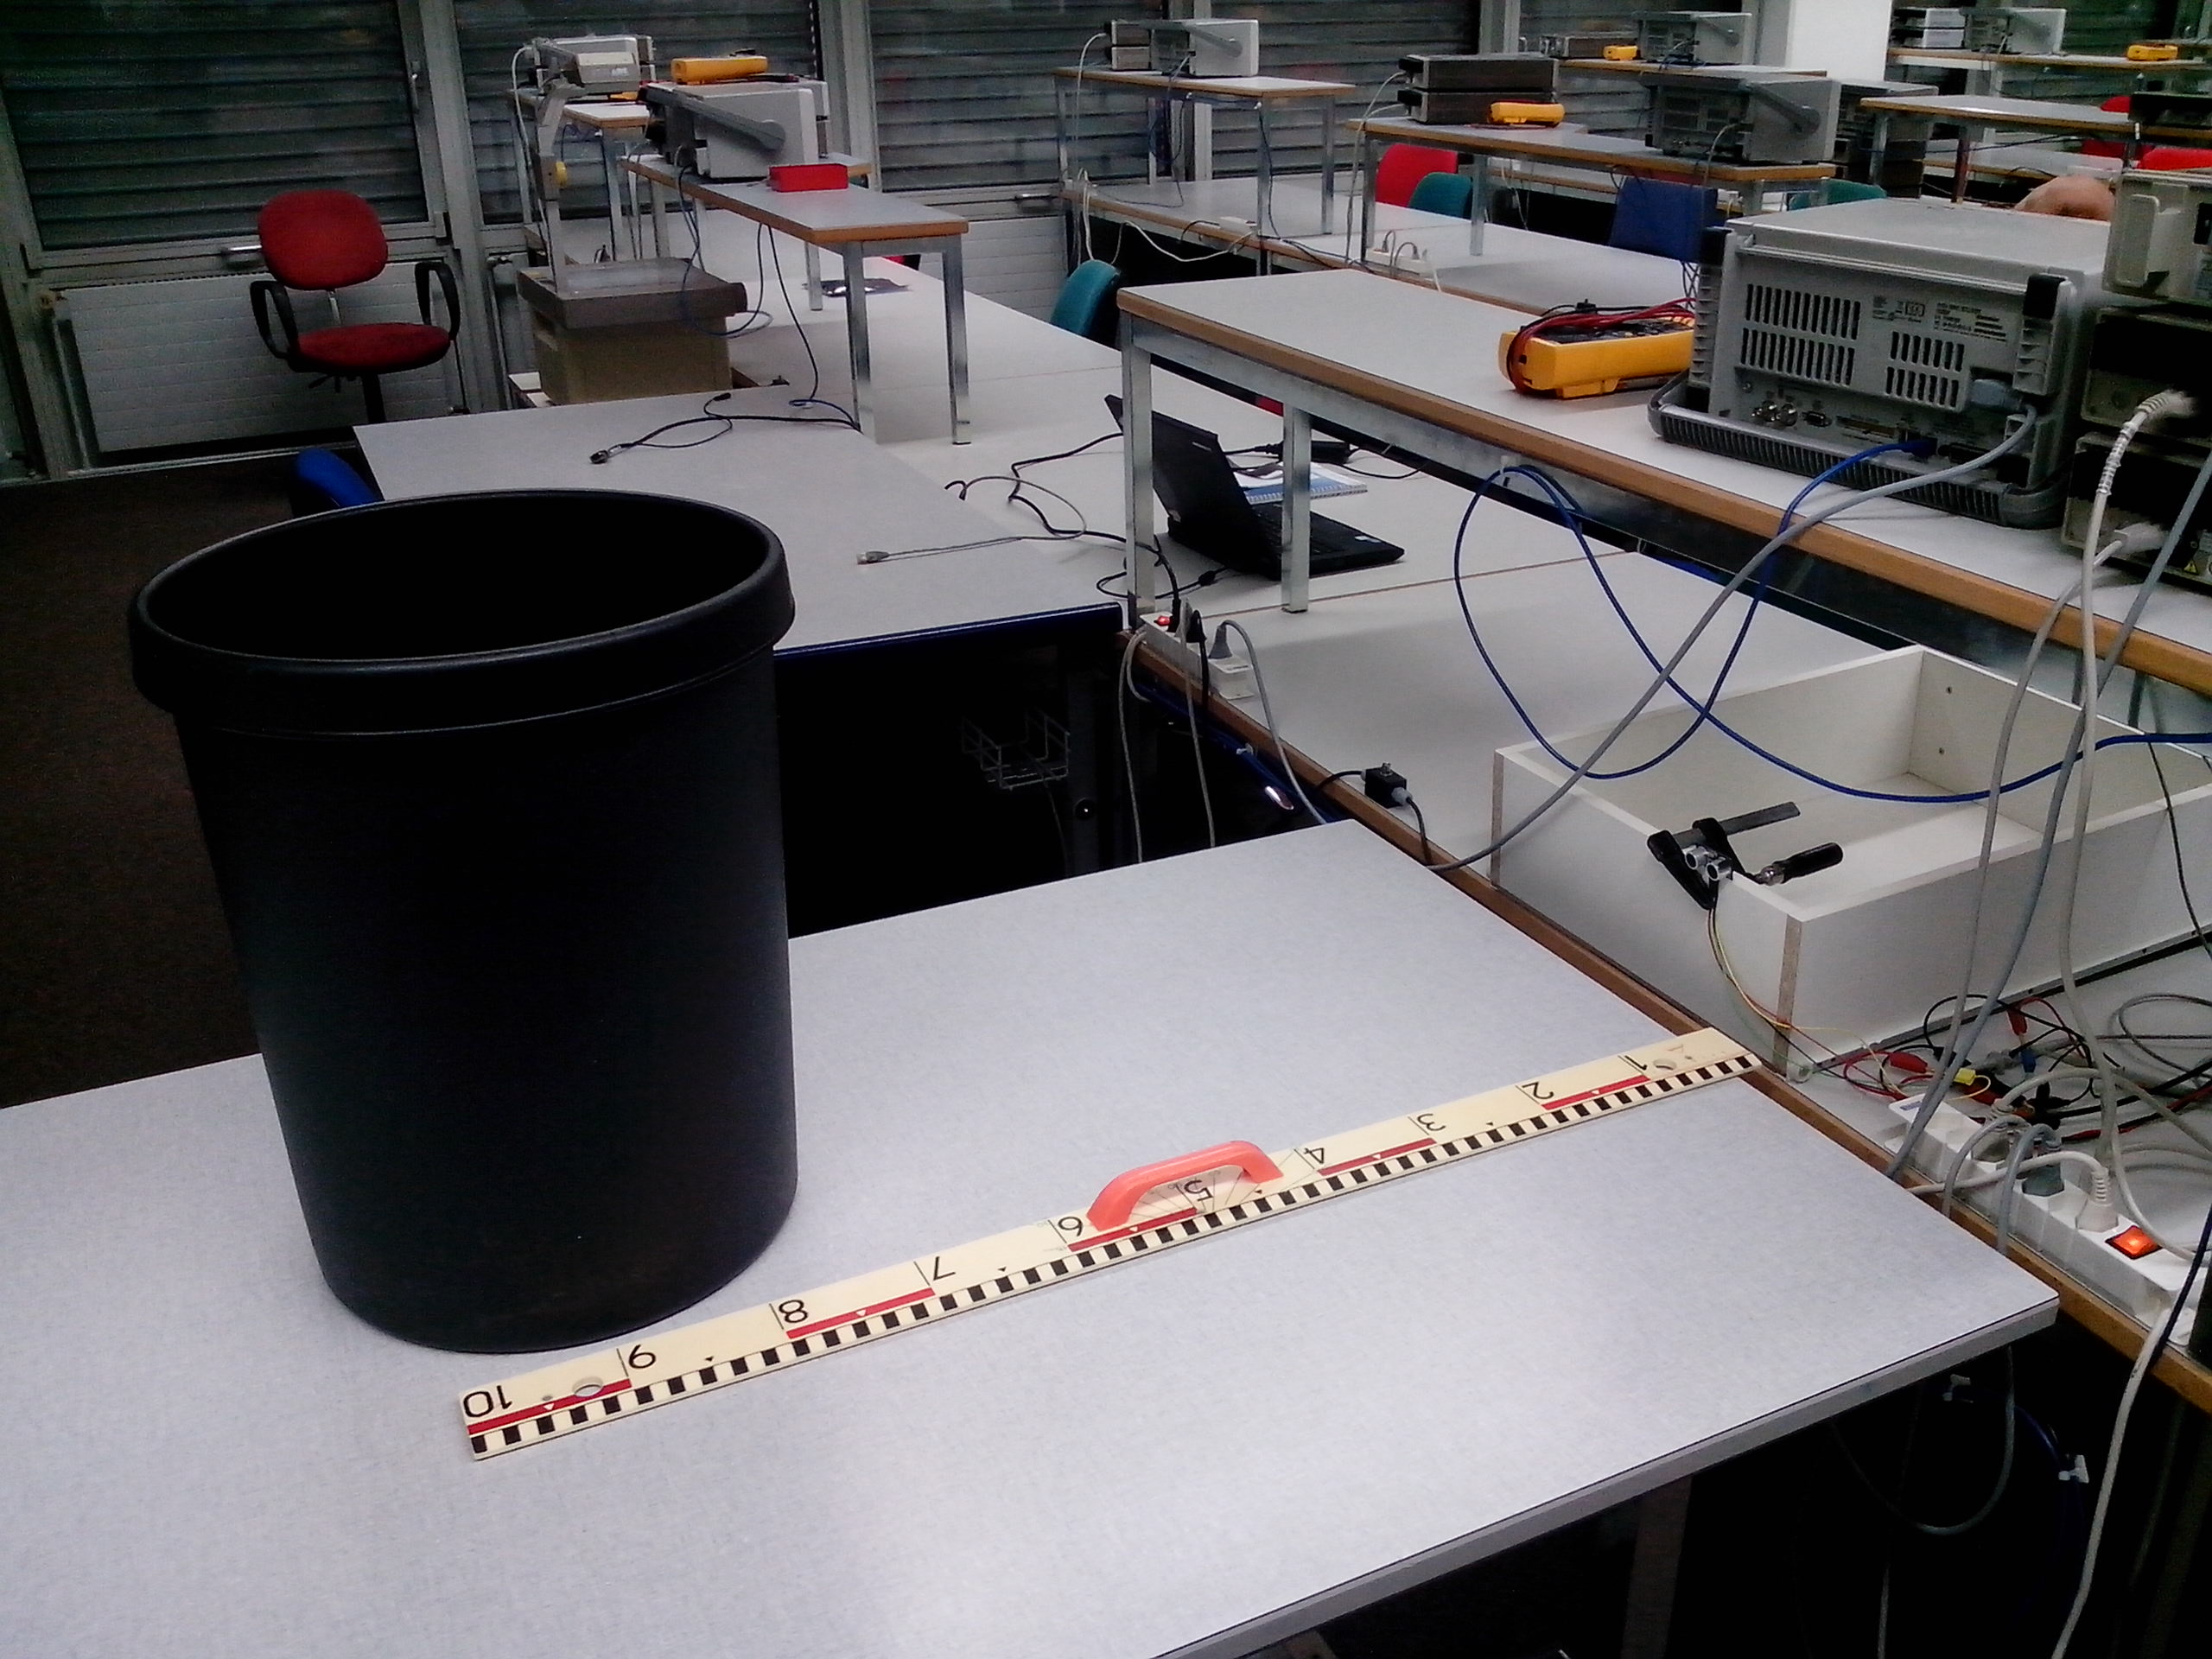
\includegraphics[width=0.5\textwidth]{../../fig/HC-SR04_01.jpg}
	\caption{Testaufbau}
	\label{fig:testaufbau_hcsr04}
\end{figure}

\subsubsection{Messgenauigkeit}
Um die Messgenauigkeit zu ermitteln ist der Testeimer dirket in Messrichtung
des Ultraschallmoduls aufgestellt worden zu verschiedenen Abständen.

\begin{comment}
\begin{table}[h!]
	\centering
	\begin{tabular}{r r r}
		$s$ [cm] & $t_i$ (mean) [ms] & $t_j$ [us] \\
		\hline
		50 	& 2.987	& 2.4 \\
		60	& 3.503 & 2.4 \\
		70	& 4.060	& 10 \\
		80	& 4.766	& 24 \\
		90	& 5.230	& 10 \\
		100	& 5.807	& 11 \\
		110	& 6.413	& 13 \\
		120	& 7.040	& 16 \\
		130	& 7.722	& 22 \\
		140	& 8.229	& 16 \\
		150	& 8.854	& 15 \\
		160	& 9.500 & 43 \\
		170	& 10.06	& 22 \\
		180	& n.a.	& n.a. \\
	\end{tabular}
	\caption{Messgenauigkeit HC-SR04}
	\label{tab:messgenauigkeit}
\end{table}
\end{comment}

\begin{figure}[h!]
	\centering
	\begin{subfigure}[b]{0.45\textwidth}
		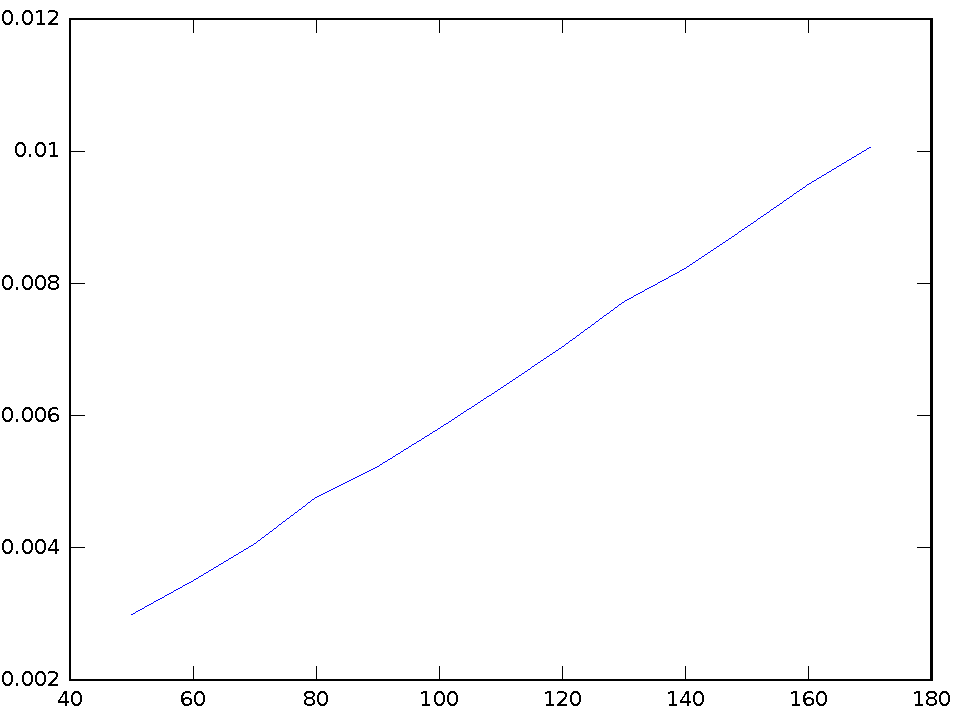
\includegraphics[width=\textwidth]{../../fig/hc-sr04_accuracy.pdf}
		\caption{Impuls Mittelwert}
	\end{subfigure}
	\begin{subfigure}[b]{0.45\textwidth}
		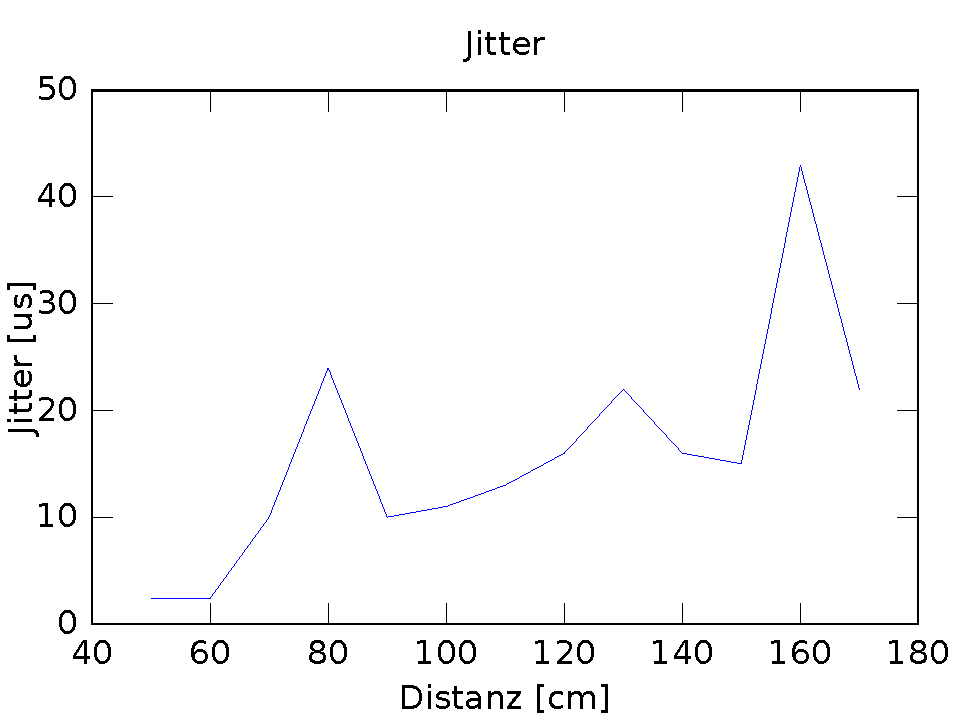
\includegraphics[width=\textwidth]{../../fig/hc-sr04_jitter.pdf}
		\caption{Jitter (Standardabweichung)}
	\end{subfigure}
	\caption{Messergebnisse der Impulsmessung}
\end{figure}

\subsubsection{Messempfindlichkeit}
